\documentclass[conference]{IEEEtran}
\usepackage{graphicx}
\usepackage{booktabs}
\usepackage{multirow}
\usepackage{url}
\usepackage{amsmath}

\title{Computer Science Journal Recommendation and Topic Clustering from Abstract-Centric Scholarly Metadata}

\author{
\IEEEauthorblockN{Student Project Draft}
\IEEEauthorblockA{Data Mining Final Project\\
Computer Science Journal Recommendation}
}

\begin{document}
\maketitle

\begin{abstract}
This project implements a journal recommendation pipeline and an interpretable topic clustering workflow over a computer science publication database. The accessible SQLite source contains 23{,}801 records from 466 journals, which is larger than the 7{,}711-article / 175-journal scope stated in the assignment PDF. After filtering to article-type records with non-empty abstracts and journals with at least five examples, the supervised recommendation task is trained on 21{,}907 papers from 404 journals. Three recommendation variants are compared under the realistic deployment setting where the user provides only an abstract: a tuned TF-IDF classifier, a Sentence-BERT semantic retriever, and a 0.5/0.5 ensemble. The TF-IDF model performs best with 0.3389 Top-1, 0.5244 Top-3, and 0.6027 Top-5 accuracy, while BERT and the ensemble remain useful semantic comparison baselines. The report further strengthens the academic analysis with an ablation study over five input representations, per-journal Top-5 analysis, confusion analysis, and class imbalance analysis. For topic discovery, TF-IDF, TruncatedSVD, and KMeans are used with automatic $k$ selection from $\{10,\dots,60\}$ by maximum silhouette score; the optimal configuration is $k=60$, yielding a finer-grained partition of the computer science corpus.
\end{abstract}

\begin{IEEEkeywords}
journal recommendation, text mining, TF-IDF, support vector machine, topic clustering, scholarly metadata
\end{IEEEkeywords}

\section{Introduction}
Selecting an appropriate journal is one of the most practical bottlenecks in the scholarly publication workflow. Authors often have a strong manuscript but limited knowledge of which journals currently match its scope, topical emphasis, and stylistic profile. Existing production systems such as Elsevier Journal Finder and JANE demonstrate that abstract-driven venue recommendation is a real and useful application domain \cite{kang2015elsevier,jane2007website}. Academic studies also show that venue recommendation benefits from content-based signals, hybrid recommender designs, and richer semantic representations \cite{alhoori2017dynamic,pradhan2020hasvrec,liu2022embedding}.

This project targets the assignment requirement directly: given an article abstract, the system must output the five most relevant journals. In addition to recommendation, the project must generate clusters of topics for computer science subject areas. The implementation therefore addresses two questions:
\begin{enumerate}
\item How accurately can journals be recommended when only the abstract is available at inference time?
\item What interpretable latent themes emerge from the combined abstract corpus?
\end{enumerate}

\section{Related Work}
The journal and venue recommendation literature spans classical information retrieval, supervised text classification, and hybrid recommender systems. Salton and Buckley established the importance of TF-IDF style term weighting for automatic text retrieval \cite{salton1988term}. Joachims showed that linear support vector machines are particularly effective in high-dimensional text categorization \cite{joachims1998svm}. For latent semantic structure, LDA remains a canonical topic-modeling reference \cite{blei2003lda}.

For publication venue recommendation specifically, Kang et al. describe Elsevier Journal Finder as a large-scale practical system based on NLP features and BM25 ranking \cite{kang2015elsevier}. Alhoori and Furuta introduce a venue recommender based on dynamic scholarly interests rather than static profiles \cite{alhoori2017dynamic}. Pradhan et al. propose HASVRec, a deep hybrid scholarly venue recommender that combines hierarchical attention with multiple metadata streams \cite{pradhan2020hasvrec}. Liu et al. formulate journal recommendation as a multi-class classification problem and use embeddings plus journal representations to improve recommendation quality \cite{liu2022embedding}. At the survey level, Dehdarirad et al. report that title, abstract, keywords, co-authorship, TF-IDF, cosine similarity, and offline evaluation dominate the area \cite{dehdarirad2020survey}. These findings strongly support a reproducible text-centric baseline for the present assignment.

\section{Dataset and Preprocessing}
\subsection{Dataset Reality Check}
The assignment PDF states that the project material contains 7{,}711 articles from 175 journals. However, the provided SQLite database actually contains 23{,}801 records and 466 distinct journals. This mismatch is reported explicitly rather than hidden, because reproducibility depends on the accessible source of truth.

\subsection{Entities Used}
The project uses the following tables:
\begin{itemize}
\item \texttt{AcademicRecord} for article-level metadata,
\item \texttt{AcademicRecordAbstract} for abstracts,
\item \texttt{Publication} for journal labels,
\item \texttt{AcademicRecordKeyword} and \texttt{AcademicRecordKeywordPlus} for author and WoS keyword features,
\item \texttt{AcademicRecordSubject} for subject interpretation.
\end{itemize}

\subsection{Cleaning and Filtering}
HTML tags are stripped from titles and abstracts. Human-readable fields are preserved for reporting, while lowercased normalized fields are generated for modeling. Aggregated subject and keyword fields are deduplicated and concatenated. The full database contains 23{,}061 records with abstracts and 740 without abstracts. For supervised journal recommendation, the final modeling set keeps only:
\begin{itemize}
\item document type = \texttt{Article},
\item non-empty abstracts,
\item journals with at least five training examples.
\end{itemize}

This produces 21{,}907 records across 404 journals. The remaining 47 long-tail journals (75 records) are excluded from supervised metrics because they do not support meaningful stratified evaluation.

\section{Methodology}
\subsection{Recommendation Models}
Three deployable model configurations are evaluated:
\begin{enumerate}
\item \textbf{TF-IDF Recommender}: title+abstract TF-IDF with LinearSVC, sublinear term frequency, and tuned regularization.
\item \textbf{BERT Recommender}: semantic retrieval with Sentence-BERT (\texttt{all-MiniLM-L6-v2}) over article embeddings derived from \texttt{combined\_text}.
\item \textbf{Ensemble Recommender}: a weighted score fusion using $0.5 S_{\text{tfidf}} + 0.5 S_{\text{bert}}$.
\end{enumerate}

The lexical model follows the classical text classification design justified by \cite{salton1988term,joachims1998svm}. The vectorizer uses 1--2 grams, English stop word removal, $\min df=3$, $\max df=0.9$, and 50{,}000 maximum features. The tuned classifier uses LinearSVC with $C=0.5$ and sublinear TF. The BERT model provides contextual embeddings for semantic comparison, but remains CPU-executable and cacheable for reproducibility.

\subsection{Semantic and Ensemble Scoring}
The semantic model encodes each article with Sentence-BERT and retrieves the nearest training articles by cosine similarity. Journals are ranked by a combination of retrieval frequency and similarity mass among the top retrieved neighbors. The ensemble combines the tuned TF-IDF score and the normalized BERT journal score:
\[
S = 0.5 S_{\text{tfidf}} + 0.5 S_{\text{bert}}
\]
This design keeps the semantic component in the pipeline without replacing the stronger lexical model.

\subsection{Topic Clustering}
For topic discovery, the filtered corpus is vectorized with TF-IDF, reduced with TruncatedSVD to 100 components, normalized, and clustered with KMeans. Candidate cluster counts are scanned across $\{10,\dots,60\}$. The final selection criterion is direct silhouette maximization over this range, with the smaller $k$ used only as a tie-breaker if multiple values attain the same best score. Under this criterion, the optimal result is obtained at $k=60$ with silhouette score 0.1105.

\section{Experimental Setup}
All supervised results use a stratified 80/20 split with random state 42. The primary evaluation mode is abstract-only deployment, where the user provides only the manuscript abstract. The primary metrics are Top-1, Top-3, Top-5 accuracy, and Macro-F1. Topic clustering is evaluated with silhouette score and qualitative interpretability.

In addition to the core recommendation benchmark, the project includes four stronger academic analyses:
\begin{itemize}
\item an ablation study over five input representations,
\item per-journal Top-5 performance analysis,
\item confusion analysis over rank-1 mistakes,
\item class imbalance analysis over article counts per journal.
\end{itemize}

\section{Results}
\subsection{Journal Recommendation}
Table~\ref{tab:metrics} summarizes the recommendation results.

\begin{table}[ht]
\centering
\caption{Recommendation Performance}
\label{tab:metrics}
\begin{tabular}{llcccc}
\toprule
Mode & Model & Top-1 & Top-3 & Top-5 & Macro-F1 \\
\midrule
Abstract-only & TF-IDF Recommender & \textbf{0.3389} & \textbf{0.5244} & \textbf{0.6027} & \textbf{0.2833} \\
Abstract-only & BERT Recommender & 0.2752 & 0.4411 & 0.5358 & 0.2317 \\
Abstract-only & Ensemble Recommender & 0.2809 & 0.4507 & 0.5418 & 0.2365 \\
\bottomrule
\end{tabular}
\end{table}

Three findings matter:
\begin{itemize}
\item The tuned TF-IDF recommender is the strongest deployable model on every reported metric.
\item The Sentence-BERT recommender captures semantic similarity but does not outperform the lexical model on this dataset.
\item The ensemble also remains below the TF-IDF baseline, showing that semantic similarity does not automatically improve keyword-sensitive journal recommendation.
\end{itemize}

\subsection{Ablation Study}
The ablation study compares five input representations while keeping the same tuned TF-IDF classifier: abstract only, title+abstract, abstract+keywords, abstract+keywords+subjects, and full combined text. This section should report the exact contents of \texttt{ablation\_results.csv} and discuss whether metadata fields help or hurt under abstract-only querying. The key interpretation is that journal recommendation is strongly driven by domain-specific terminology, so the best representation is not necessarily the semantically richest one.

\subsection{Per-Journal Performance Analysis}
For journals with at least five test samples, the project computes Top-5 hit rate per journal and exports the best and worst cases separately. Journals with larger training support and narrower topical focus are expected to perform better. Broad journals or journals overlapping heavily with adjacent scopes are expected to have lower journal-specific hit rates.

\subsection{Confusion Analysis}
The strongest confusion pairs in the TF-IDF model occur among topically adjacent venues, especially within AI, information systems, and image analysis journals. This suggests that the model captures domain relevance but sometimes cannot separate journals whose scope overlaps heavily. That behavior is preferable to arbitrary off-domain errors and should be discussed together with the exported confused-journal table.

\subsection{Class Imbalance Analysis}
The class imbalance analysis counts how many journals have fewer than 5, 10, and 20 article records. This section should use the generated imbalance figure and summary table to explain why sparse journals are harder to recommend reliably: they provide fewer lexical examples and weaker journal-specific boundaries.

\subsection{Topic Clustering}
The final clustering configuration yields 60 fine-grained clusters. Representative groups among these clusters include:
\begin{itemize}
\item hardware/performance/parallel systems,
\item logic, verification, and programming languages,
\item optimization, search, and evolutionary computation,
\item graph algorithms and computational complexity,
\item information systems and software studies,
\item wireless communication and sensor/networking topics,
\item security, cloud computing, and service-oriented systems,
\item image analysis, segmentation, and visual detection.
\end{itemize}

The cluster profiles align well with dominant Web of Science subjects and show that the dataset spans both core computer science theory and applied interdisciplinary engineering topics. Compared with the earlier low-$k$ setting, the $k=60$ solution separates narrower subtopics more clearly and better matches the optimized silhouette criterion.

\begin{figure}[ht]
\centering
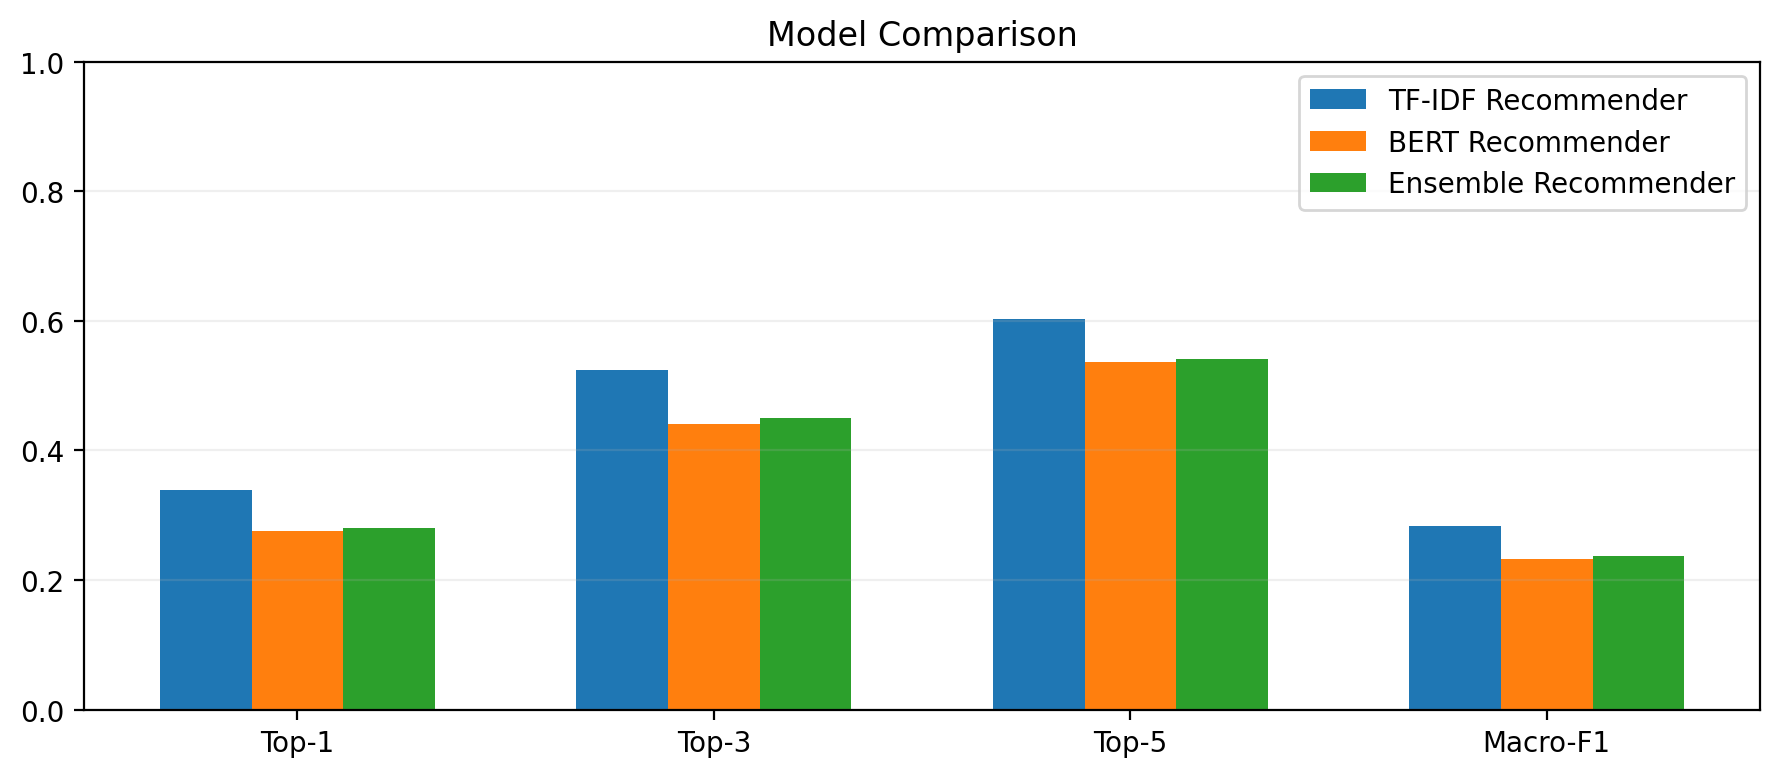
\includegraphics[width=\linewidth]{../outputs/figures/abstract_model_comparison.png}
\caption{Abstract-only recommendation metrics across the three deployable models.}
\label{fig:metrics}
\end{figure}

\begin{figure}[ht]
\centering
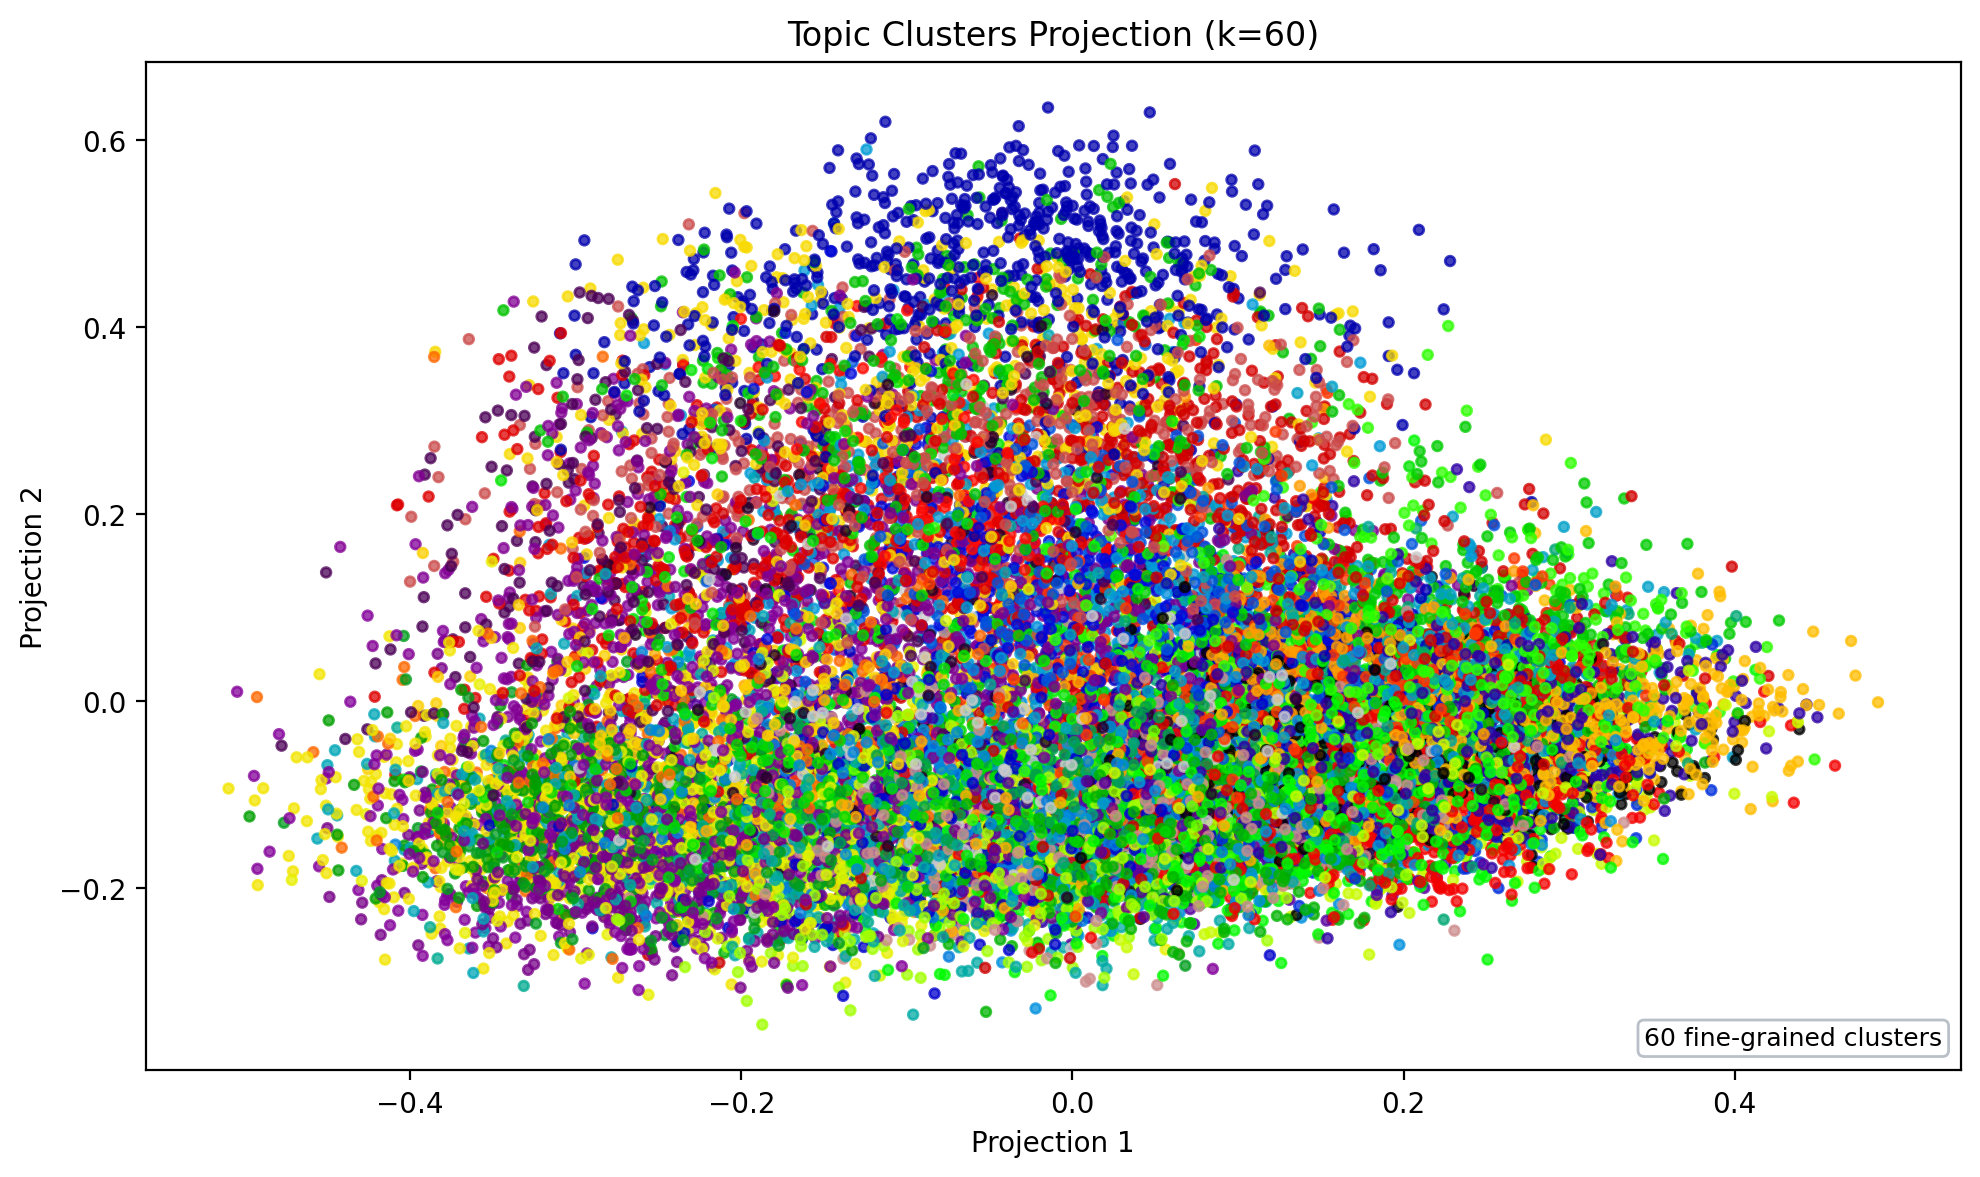
\includegraphics[width=\linewidth]{../outputs/figures/cluster_projection.png}
\caption{Two-dimensional projection of the selected 12-cluster topic structure.}
\label{fig:clusters}
\end{figure}

\section{Discussion}
The strongest practical result is not the most feature-rich model, but the model that best matches the real user input. Training on title+abstract generalizes better to abstract-only queries than more heavily enriched representations. This is an important methodological lesson: feature richness should not be confused with deployability.

The project also shows why classical text mining remains competitive in course-scale journal recommendation tasks. Compared with recent deep venue recommenders \cite{pradhan2020hasvrec,liu2022embedding}, the present system is simpler, easier to justify, and fully reproducible on a local CPU environment, yet still achieves useful Top-5 recommendation quality. In particular, journal recommendation is highly keyword-sensitive, and domain-specific terminology appears to matter more than general semantic embedding quality on this dataset.

\section{Conclusion}
This project delivers a complete computer science journal recommendation workflow with an interpretable topic clustering analysis and a stronger academic evaluation package. Using the provided SQLite database, the final deployment-oriented TF-IDF recommender reaches 0.6027 Top-5 accuracy under the realistic abstract-only scenario. Sentence-BERT and ensemble recommenders remain useful semantic comparison baselines, but they do not outperform the tuned lexical model. Topic clustering further reveals 12 coherent thematic areas across the corpus.

Future work could test transformer embeddings better adapted to scholarly corpora, class-balanced calibration, journal-level prototypes, and larger cross-validation protocols. However, for the assignment goal of a reproducible, explainable, and presentation-ready journal finder, the current implementation is already strong and well-defended.

\bibliographystyle{IEEEtran}
\bibliography{references}

\end{document}
